\documentclass[11pt]{book}
\usepackage{amsmath,amssymb,graphicx}
\usepackage{../setspace}
\usepackage{color}
\addtolength{\textwidth}{1.5in}
\addtolength{\hoffset}{-1in}
\addtolength{\textheight}{1.5in}
\addtolength{\voffset}{-1in}
\usepackage{/usr/share/R/share/texmf/Sweave}

\title{STAT3401 Multivariate Lab Workbook}
\author{Paul Hewson}
\begin{document}
\setlength{\parindent}{0pt}
\setlength{\parskip}{12pt}
\sffamily



\maketitle


\chapter*{Introduction}

Hello and welcome to the multivariate statistics part of STAT3401.   One word of caution about these notes.   The first column of the notes will have either a $>$ or a $+$ symbol denoting the R prompt or the ``R command carrying over an additional line''.   You don't need to type that in.  

I might put some of the longer R functions in the portal, to save a little typing.   Nevertheless, you do need to \emph{understand} what you are doing.


\chapter{Week 1: EDA}

Monday 28th September

\input{week1eda}

\chapter{Week 2: Matrices}

Monday 5th October



\section{Computer exercises for the lab}

This week is a good time for
\begin{itemize}
\item[(a)] making sure you are comfortable with the mathematics behind matrices as well as:
\item[(b)] making sure you are comfortable with the matrix operators in R.   
\item[(c)]  Check that you are very very sure you can subscript R matrices, i.e. use things such as \text{[,1]} to select column 1, \text{[,-1]} to select everything \emph{except} column 1, and \text{[,2:3]} to select columns 2 and 3.
\end{itemize}

Although we will use in built multivariate analysis functions in R, you should consider checking you understand the techniques by using R as a matrix calculator.
  
\begin{enumerate}

\item Find (where possible) the determinants and the inverse of the following matrices:

$C_{1} = \left[ \begin {array}{cc} 4& 4\\\noalign{\medskip} 4& 4\end {array} \right]$, $C_{2} = \left[ \begin {array}{cc} 4& 4.001\\\noalign{\medskip} 4.001& 4.002\end {array} \right]$ and $C_{3} = \left[ \begin {array}{cc} 4& 4.001\\\noalign{\medskip} 4.001& 4.002001\end {array} \right] $

Very briefly comment on the magnitude of the difference between $C_{2}^{-1}$ and  $C_{3}^{-1}$ given the only difference between $C_{2}$ and $C_{2}$ amounts to a difference of $0.000001$ in the bottom right position.

\begin{Schunk}
\begin{Sinput}
> A <- matrix(c(4, 4, 4, 4), 2, 2)
> A
> det(A)
> try(solve(A))
> B <- matrix(c(4, 4.001, 4.001, 4.002), 2, 2)
> B
> det(B)
> solve(B)
> C <- matrix(c(4, 4.001, 4.001, 4.002001), 2, 2)
> C
> det(C)
> solve(C)
\end{Sinput}
\end{Schunk}


\begin{itemize}
  \item What's going on here?
\end{itemize}

\textit{Note that A is singular, the determinant is zero and it can't be inverted.   Also note that the inverses of B and C are very very different - but this is something of a pathological example}


\item Matrix partitioning.   Consider Sterling's financial data held in the R object LifeCycleSavings (see \verb+?LifeCycleSavings+).   To make life a little easier, reorder the columns using \texttt{X <- LifeCycleSavings[,c(2,3,1,4,5)]}.
  

\begin{itemize}
\item Find the correlation matrix of \texttt{X} (longhand, using the centering matrix), call this matrix \texttt{R}


\begin{Schunk}
\begin{Sinput}
> data(LifeCycleSavings)
> X <- LifeCycleSavings[, c(2, 3, 1, 4, 5)]
> R <- cor(X)
> R
\end{Sinput}
\end{Schunk}


\item Partition \textit{R = cov(X)} following the scheme below such that $\boldsymbol{R_{11}}$ is a $2 \times 2$ matrix containing the covariance of \texttt{pop15} and \texttt{pop75}, and $\boldsymbol{R_{22}}$ contains the covariance of \texttt{sr}, \texttt{dpi} and \texttt{ddpi}

\begin{displaymath}
\boldsymbol{R} = \left( \begin{array}{l|l} \boldsymbol{R_{11}} & \boldsymbol{R_{12}} \\ \hline    \boldsymbol{R_{21}} & \boldsymbol{R_{22}} \end{array} \right) 
\end{displaymath}

You should find for example that  $\boldsymbol{R_{11}}$ is given by:
 % latex table generated in R 2.3.1 by xtable 1.3-2 package
% Wed Nov 15 22:15:30 2006
\begin{table}[ht]
\begin{center}
\begin{tabular}{rrr}
\hline
 & pop15 & pop75 \\
\hline
pop15 & 83.75 & $-$10.73 \\
pop75 & $-$10.73 & 1.67 \\
\hline
\end{tabular}
\end{center}
\end{table}

\begin{Schunk}
\begin{Sinput}
> R11 <- R[1:2, 1:2]
> R12 <- R[1:2, 3:5]
> R21 <- R[3:5, 1:2]
> R22 <- R[3:5, 3:5]
> R11
> R22
> R21
> R12
> t(R21)
\end{Sinput}
\end{Schunk}


\item Find the matrix $\boldsymbol{A}$, where:

\begin{displaymath}
\boldsymbol{A} = \boldsymbol{R_{22}^{-1}R_{21}R_{11}^{-1}R_{12}}
\end{displaymath}



\begin{Schunk}
\begin{Sinput}
> A <- solve(R22) %*% R21 %*% solve(R11) %*% R12
\end{Sinput}
\end{Schunk}


%\begin{itemize}

\item Are $\boldsymbol{A}$ and $\boldsymbol{B}$ symmetric?   What is the difference between symmetric and asymmetric matrices in terms of their eigenvalues and eigenvectors?\\
\textit{Note that they are both asymmetric matrices, it just so happens for these particular matrices that the eigenvalues are positive and the eigenvectors are real.   This isn't always the case for asymmetric matrices!}

\item Find the eigenvalues and eigenvectors of $\boldsymbol{A}$ and $\boldsymbol{B}$ then find the square roots of the eigenvalues.   


\begin{Schunk}
\begin{Sinput}
> eigen(B)
> sqrt(eigen(A)$values)
> sqrt(eigen(B)$values)
\end{Sinput}
\end{Schunk}


\item Do you notice any similarities between the first two eigenvalues from either matrix?\\
\textit{Note that the square roots of the eigen values are identical.}
\end{itemize}

\item Revisit the \texttt{wines} data in the \texttt{Flury} package.   Consider only Y1, Y5, Y6, Y8 and Y9, use matrix algebra to find the means, correlation and covariance of these data.   Compare the eigenvalues and eigenvectors, and the determinants and inverse you get from the covariance matrix and the correlation matrix.\\


  
  
\end{enumerate} 


\section{Summary of week 2}

\fbox{\parbox[c]{0.9\textwidth}{\color{blue}
    
\begin{itemize}
\item We have revised, and are comfortable with matrix multiplication, matrix inverse, (normalised) eigenvalues and eigenvectors.  We can center and scale matrices.  We can do this by hand and in R.
\item We are also comfortable using R as a matrix calculator if and when we wish.
\end{itemize}
}}


\chapter{Week 3: Distance measures}

Monday 12th October

\input{week3Distance}

\chapter{Week 4: Cluster analysis}

Monday 19th October

\input{week4cluster}

\chapter{Week 5: Principal components analysis}

Monday 26th October

\input{week5pca}

%\chapter{Week 6: Self Study (Canonical Correlation)}

%\chapter{Canonical Correlation}
\label{cancor}

\section{Canonical variates}
\label{canvar}

\section{Interpretation}
\label{canint}
%%%%%\chapter{Canonical Correlation}

In canonical correlation, we are interested in the relationship between two sets of variables.   We do this by creating linear combinations $\boldsymbol{U} = \boldsymbol{a_{1} x_{1}} + \boldsymbol{a_{2} x_{2}} + \cdots + \boldsymbol{a_{p} x_{p}}$ and  $\boldsymbol{V} = \boldsymbol{b_{1} y_{1}} + \boldsymbol{b_{2} y_{2}} + \cdots + \boldsymbol{b_{q} y_{q}}$ such that the correlation between $\boldsymbol{U}$ and $\boldsymbol{V}$ is as high as possible.


To do this, we need to work out the correlation matrix, and partition it:


\begin{displaymath}
\begin{array}{ccccccc} & x_{1} & \ldots & \_{p} & y_{1} & \ldots & y_{q} \end{array}
\end{displaymath}
\begin{displaymath}
\begin{array}{c} x_{1} \\ \vdots \\ x_{p} \\y_{1} \\ \vdots \\y_{3}\end{array}
\left( \begin{array}{ccc|ccc} &&&&&\\&A_{p \times p}& &C_{p \times q}&\\&&&&&\\
\hline
&&&&&\\&C_{q \times p}& &B_{q \times q}&\\&&&&&\\ \end{array} \right)
\end{displaymath}

Having done this, we calculate the matrix:

\begin{displaymath}
\boldsymbol{B^{-1}C^{T}A^{-1}C}
\end{displaymath}

and find the associated eigenvalues (in descending order)  $\lambda_{1} > \lambda_{2} > \ldots > \lambda_{r}$.   The corresponding eigenvectors $\boldsymbol{b_{1}}, \boldsymbol{b_{2}}, \ldots, \boldsymbol{b_{r}}$ give the coefficients of the Y variables.

So: 

\begin{displaymath}
\boldsymbol{v_{i}} = \boldsymbol{b_{i}^{T}} \boldsymbol{Y}
\end{displaymath}

where $\boldsymbol{b_{i}} = \left(\begin{array}{c} b_{i1} \\ \vdots \\ b_{iq} \end{array} \right)$ and $\boldsymbol{Y} = \left(\begin{array}{c} \boldsymbol{y_{1}} \\ \vdots \\ \boldsymbol{y_{q}} \end{array} \right)$, or in longhand:

\begin{displaymath}
\boldsymbol{v_{i}} = b_{i1} \boldsymbol{y_{1}} + \cdots + b_{iq} \boldsymbol{y_{q}}
\end{displaymath}

Having calculated these, it is possible to solve the coefficients for the X variables:

$a_{1} = \boldsymbol{A^{-1} C b_{1}}, a_{2} = \boldsymbol{A^{-1} C b_{2}}, \ldots,  a_{r} = \boldsymbol{A^{-1} C b_{r}}$,

f
\begin{displaymath}
\boldsymbol{u_{i}} = \boldsymbol{a_{i}^{T}} \boldsymbol{X}
\end{displaymath}


where $\boldsymbol{a_{i}} = \left(\begin{array}{c} a_{i1} \\ \vdots \\ a_{iq} \end{array} \right)$ and $\boldsymbol{X} = \left(\begin{array}{c} \boldsymbol{x_{1}} \\ \vdots \\ \boldsymbol{x_{r}} \end{array} \right)$, or in longhand:

\begin{displaymath}
\boldsymbol{u_{i}} = a_{i1} \boldsymbol{x_{1}} + \ldots + a_{ir} \boldsymbol{x_{r}}
\end{displaymath}

And one really cute result is that $\left[corr(\boldsymbol{u_{i}}, \boldsymbol{v_{i}})\right]^{2} = \lambda_{i}$.

\section{Computer example}

Franco Modigliani proposed a life cycle savings model, the savings ratio (aggregate personal saving divided by disposable income) is explained by per-capita disposable income, the percentage rate of change in per-capita disposable income, and two demographic variables: the percentage of population less than 15 years old and the percentage of the population over 75 years old. 

However, we are interested here in the relationship between the two demographic variables (percent of population under 15, percent of population over 75) and the three financial variables (personal savings, per-capita disposal income, growth rate of dpi).   The first stage of any such analysis would be a visual inspection.


\begin{verbatim}
pairs(LifeCycleSavings, pch = 16)
\end{verbatim}

\begin{figure}
\begin{center}
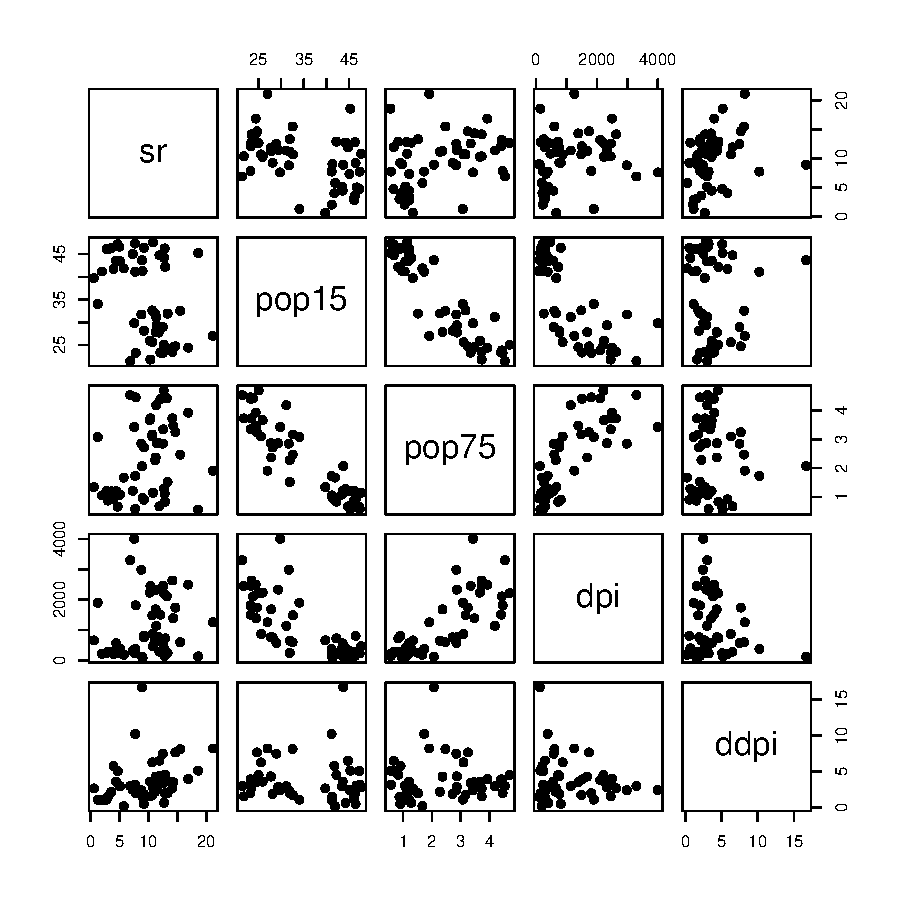
\includegraphics[width = 0.6\textwidth]{images/cancor}
\caption{Pairwise scatterplots of Life Cycle Savings data}
\end{center}
\end{figure}

And it is worth examining the correlation matrix:

\singlespacing
\begin{verbatim}
> cor(LifeCycleSavings)
              sr       pop15       pop75        dpi        ddpi
sr     1.0000000 -0.45553809  0.31652112  0.2203589  0.30478716
pop15 -0.4555381  1.00000000 -0.90847871 -0.7561881 -0.04782569
pop75  0.3165211 -0.90847871  1.00000000  0.7869995  0.02532138
dpi    0.2203589 -0.75618810  0.78699951  1.0000000 -0.12948552
ddpi   0.3047872 -0.04782569  0.02532138 -0.1294855  1.00000000
\end{verbatim}
\onehalfspacing

It appears that the \textbf{X} variables are correlated.   This is less so for \textbf{Y} variables, and even less so for \textbf{X,Y} inter-correlations.

You need to be sure that the variables are \emph{scaled} before carrying out a canonical correlation analysis.   

\singlespacing
\begin{verbatim}
LifeCycleSavingsS <- scale(LifeCycleSavings)
pop <- LifeCycleSavingsS[, 2:3] ## The X matrix
oec <- LifeCycleSavingsS[, -(2:3)] ## the Y matrix
\end{verbatim}
\onehalfspacing

Having created an \textbf{X} matrix and a \textbf{Y} matrix, we now want to find linear combinations of \textbf{X} which have maximum correlation with \textbf{Y}.

\singlespacing
\begin{verbatim}
> cancor(pop, oec)
$cor
[1] 0.8247966 0.3652762

$xcoef
             [,1]       [,2]
pop15 -0.08338007 -0.3314944
pop75  0.06279282 -0.3360027

$ycoef
           [,1]        [,2]         [,3]
sr   0.03795363  0.14955310 -0.023106040
dpi  0.12954600 -0.07518943  0.004502216
ddpi 0.01196908 -0.03520728  0.148898175

$xcenter
        pop15         pop75 
-4.662937e-16  2.753353e-16 

$ycenter
          sr          dpi         ddpi 
1.421085e-16 6.661338e-17 4.440892e-16 
\end{verbatim}
\onehalfspacing

This indicates one canonical correlate with a correlation of 0.8247966 between $z_{\boldsymbol{X}1}$ and $z_{\boldsymbol{Y}1}$

\begin{eqnarray}
z_{\boldsymbol{X}1} =  -0.08338007  x_{pop15} + 0.06279282 x_{pop75}\\
z_{\boldsymbol{Y}1} = 0.03795363 y_{sr} + 0.12954600 y_{dpi} +  0.01196908 y_{ddpi}
\end{eqnarray}

If we extract the coefficients as vectors (this time we have created \texttt{LCS.cancor} as an object; also we have used \texttt{as.numeric(\ldots)} to extract the coefficients in a form suitable for matrix multiplication).

\singlespacing
\begin{verbatim}
> LCS.cancor <- cancor(pop, oec)
> ycoef <- as.numeric(LCS.cancor$ycoef[,1])
> xcoef <- as.numeric(LCS.cancor$xcoef[,1])
> v1 <-  oec %*% ycoef ## remember oec and pop are scaled
> u1 <-  pop %*% xcoef
> plot(v1, u1)
> identify(v1, u1, row.names(LifeCycleSavings))
\end{verbatim}
\onehalfspacing


\subsection{Interpreting the canonical variables}

There is some ``controversy'' about the best way of interpreting the canonical variables.   You have two possibilities:

\begin{itemize}
\item Interpret the coefficients in a similar way to that used in principal components (problems with collinear variables)
\item Calculate the correlation between the canonical and the original variables (doesn't tell you anything about joint contributions)
\end{itemize}

%Consider:

%$\rho_{\hat{U},\boldsymbol{x}}$ = matrix of correlations between $\hat{U}$ and $\boldsymbol{x}$\\ 
%$\rho_{\hat{V},\boldsymbol{y}}$ = matrix of correlations between $\hat{V}$ and $\boldsymbol{y}$ \\
%$\rho_{\hat{U},\boldsymbol{y}}$ = matrix of correlations between $\hat{U}$ and $\boldsymbol{y}$ \\
%$\rho_{\hat{V},\boldsymbol{x}}$ = matrix of correlations between $\hat{V}$ and $\boldsymbol{x}$\\ 

%Which can be obtained fairly simply as:

%\begin{eqnarray*}
%\rho_{\hat{U},\boldsymbol{x}} = a \Sigma_{11}



\subsection{Hypothesis testing}

As with Principal Components, a certain amount of hypothesis testing is possible.   The distributional properties of canonical variables is far wilder than principal components - none of the recommended books discuss it.   However, the tests can be described.   For example, if we wanted to test whether there was any relationship between our two sets of variables:

\begin{displaymath}
H_{0}; \boldsymbol{\Sigma}_{12} = \boldsymbol{0}
\end{displaymath}

The Likelihood ratio test leads us to:

\begin{displaymath}
\Lambda^{\frac{2}{n}} = |\boldsymbol{I} - \boldsymbol{S_{22}^{-1}}\boldsymbol{S_{21}}\boldsymbol{S_{11}^{-1}}\boldsymbol{S_{12}}| = \prod_{i=1}^{k}(1-r_{i}^{2}) \sim \Lambda_{Wilks}(p, n-1-q,q)
\end{displaymath}

Using Bartlett's approximation this can yield a $chi^{2}$ test:

\begin{displaymath}
-\left(n-\frac{1}{2}(p+q+3)\right) \log \prod_{i=1}^{k}(1-r_{i}^{2}) \sim \chi^{2}_{pq}
\end{displaymath}


As we've seen before, perhaps we are more interested in finding out how many canonical correlations we need to keep in our analysis.   Bartlett also proposed a statistic only $s$ canonical correlations are non-zero:

\begin{displaymath}
-\left(n-\frac{1}{2}(p+q+3)\right) \log \prod_{i=s+1}^{k}(1-r_{i}^{2}) \sim \chi^{2}_{(p-s)(q-s)}
\end{displaymath}

%%% Local Variables: ***
%%% mode:latex ***
%%% TeX-master: "book.tex"  ***
%%% End: ***

\chapter{Week 6: Hotelling's test}

Monday 2nd November



\section{Two sample Hotelling's T$^{2}$ test}

We are going to consider an example using data from Flea Beetles reported by Lubischew (1962) and used in Flury (1997).  We are going to use \textbf{R} as a sophisticated calculator and work through a lot of the calculations long hand first.

\begin{Schunk}
\begin{Sinput}
> library(Flury)
> `?`(flea.beetles)
> data(flea.beetles)
\end{Sinput}
\end{Schunk}


It can be seen that there is a factor ``Species'' denoting whether the beetles are from 'oleracea' or 'carduorum'.   There are four numeric variables as follows: 'TG'; Distange of the Transverse Groove to the posterior border of
          the prothorax (microns), 'Elytra'; Length of the Elytra (in units of 0.01mm), 'Second.Antenna'; Length of the second antennal joint (microns) and 'Third.Antenna'; Length of the third antennal joint (microns).   We need to estimate the mean for each sample, and calculate the difference between the two vectors:

\begin{Schunk}
\begin{Sinput}
> mu <- by(flea.beetles[, -1], flea.beetles$Species, colMeans)
> mudiff <- mu[[1]] - mu[[2]]
> p <- dim(flea.beetles)[2] - 1
\end{Sinput}
\end{Schunk}

The next step is to extract the two covariance matrices:

\begin{Schunk}
\begin{Sinput}
> covmats <- by(flea.beetles[, -1], flea.beetles$Species, cov)
> covmats
\end{Sinput}
\begin{Soutput}
flea.beetles$Species: oleracea
                      TG    Elytra Second.Antenna Third.Antenna
TG             187.59649 176.86257       48.37135     113.58187
Elytra         176.86257 345.38596       75.97953     118.78070
Second.Antenna  48.37135  75.97953       66.35673      16.24269
Third.Antenna  113.58187 118.78070       16.24269     239.94152
------------------------------------------------------------ 
flea.beetles$Species: carduorum
                      TG    Elytra Second.Antenna Third.Antenna
TG             101.83947 128.06316       36.98947      32.59211
Elytra         128.06316 389.01053      165.35789      94.36842
Second.Antenna  36.98947 165.35789      167.53684      66.52632
Third.Antenna   32.59211  94.36842       66.52632     177.88158
\end{Soutput}
\end{Schunk}


and then to estimate the pooled covariance matrix $\boldsymbol{S}$ for the flea beetle data (where N[1] gives $n_{1}$,  N[2] gives $n_{2}$), can be calculated as:

\begin{Schunk}
\begin{Sinput}
> N <- xtabs(~flea.beetles[, 1])
> pooledS <- ((N[1] - 1) * covmats[[1]] + (N[2] - 1) * covmats[[2]])/(N[1] + 
+     N[2] - 2)
> pooledS
\end{Sinput}
\begin{Soutput}
                      TG   Elytra Second.Antenna Third.Antenna
TG             143.55910 151.8034       42.52660      71.99253
Elytra         151.80341 367.7878      121.87653     106.24467
Second.Antenna  42.52660 121.8765      118.31408      42.06401
Third.Antenna   71.99253 106.2447       42.06401     208.07290
\end{Soutput}
\begin{Sinput}
> Sinv <- solve(pooledS)
> Sinv
\end{Sinput}
\begin{Soutput}
                         TG        Elytra Second.Antenna Third.Antenna
TG              0.013257964 -0.0053492256   0.0015134494 -0.0021617878
Elytra         -0.005349226  0.0066679441  -0.0047337699 -0.0005969439
Second.Antenna  0.001513449 -0.0047337699   0.0130490933 -0.0007445297
Third.Antenna  -0.002161788 -0.0005969439  -0.0007445297  0.0060093005
\end{Soutput}
\end{Schunk}


Having calculated the inverse of the pooled correlation matrix we also need the scaling factor $\frac{n_{1} n_{2}}{n_{1} + n_{2}}$.   Hotellings T$^{2}$ is then quite straightforward to calculate:


\begin{Schunk}
\begin{Sinput}
> scaleFact <- (N[1] * N[2])/(N[1] + N[2])
> Hotellings <- t(mudiff) %*% Sinv %*% mudiff * scaleFact
> Hotellings
\end{Sinput}
\begin{Soutput}
         [,1]
[1,] 133.4873
\end{Soutput}
\end{Schunk}


which is the value of the T$^{2}$ statistic.   We could work with this value directly, but it is more convenient to transform it into something we can compare with the $F$ distribution.

\begin{Schunk}
\begin{Soutput}
       [,1]
[1,] 30.666
\end{Soutput}
\end{Schunk}


and we compare this with an $F$ distribution having $p$ and $(n_{1} + n_{2} - p - 1)$ d.f.

And we can check this as follows:

\begin{Schunk}
\begin{Sinput}
> pf(test, p, N[1] + N[2] - p - 1, lower.tail = FALSE)
\end{Sinput}
\end{Schunk}

which gives us the area under the curve from our test statistic ($30.666$) to $\infty$.   Clearly in this case, we have reject H$_{0}$, i.e. there is evidence that the mean vectors, $\bar{\boldsymbol{x}}_{oleracea} = (194.4737, 267.0526, 137.3684, 185.9474)$, $\bar{\boldsymbol{x}}_{carduorum} = (179.55, 290.80, 157.20, 209.25)$, 
 for the two species differ.   This is perhaps no surprise if you consider the data - do look at the scatterplot suggested by the helpfile.

\begin{itemize}
\item How would you modify the code to carry out a one sample T$^{2}$ test?
\item You may wish to repeat this exercise with the \texttt{turtles} data.   
\end{itemize}

You also should note that in practice this calculation is done my means of the QR decomposition, details are given in Seber (1984).   There is no in-built \textbf{R} function for doing these calculations - a nice little project for someone.   The \texttt{manova()} function can be persuaded to carry out a two sample Hotelling's T$^{2}$ test as follows:

\begin{Schunk}
\begin{Sinput}
> hotel.test <- manova(as.matrix(flea.beetles[, -1]) ~ flea.beetles[, 
+     1])
> summary(hotel.test, test = "Hotelling")
\end{Sinput}
\end{Schunk}

\section{Drawing the ellipses}


This illustration is based on, but differs from code provided by Marco Bee to accompany Flury (1997).   Firstly, we need a function to draw ellipses:

\begin{Schunk}
\begin{Sinput}
> ellipse <- function(covmat, centroid, csquare, resolution, plot = TRUE) {
+     angles <- seq(0, by = (2 * pi)/resolution, length = resolution)
+     sd <- covmat[1, 2]/sqrt(covmat[1, 1] * covmat[2, 2])
+     projmat <- matrix(0, 2, 2)
+     projmat[1, 1] <- sqrt(covmat[1, 1] %*% (1 + sd)/2)
+     projmat[1, 2] <- -sqrt(covmat[1, 1] %*% (1 - sd)/2)
+     projmat[2, 1] <- sqrt(covmat[2, 2] %*% (1 + sd)/2)
+     projmat[2, 2] <- sqrt(covmat[2, 2] %*% (1 - sd)/2)
+     circle <- cbind(cos(angles), sin(angles))
+     ellipse <- t(centroid + sqrt(csquare) * projmat %*% t(circle))
+     if (plot == TRUE) {
+         lines(ellipse)
+     }
+     return(ellipse)
+ }
\end{Sinput}
\end{Schunk}

It is possible to define a function which calculates $c^{2}$ and calls the ellipse routine (I'm not completely convinced this is doing the calculation correctly yet, in particular I'm not sure I'm using the correct tail).

\begin{Schunk}
\begin{Sinput}
> mean.ellipse <- function(data, alpha = 0.05, resolution = 500) {
+     xbar <- colMeans(data)
+     n <- dim(data)[1]
+     p <- dim(data)[2]
+     f <- qf(1 - alpha, p, n - p)
+     csquare <- ((n - 1)/n) * (p/(n - p)) * f
+     cat(csquare)
+     ellipse <- ellipse(cov(data), xbar, csquare, resolution)
+ }
\end{Sinput}
\end{Schunk}

%# call procedure ellips

%X <- ellips(A, m, const, k)               

%# graph the results

For illustrative purposes, we'll create a $n \times 2$ data object from our flea beetles.   Do note here that we are \emph{only} using two variables!



Given the above functions, it is quite straightforward to plot the centroids and constant density ellipses:

\begin{Schunk}
\begin{Sinput}
> X <- cbind(flea.beetles[, 2], flea.beetles[, 3])
> plot(X)
> points(t(colMeans(X)), pch = 16, col = "red")
> mean.ellipse(X, alpha = 0.01)
> mean.ellipse(X, alpha = 0.05)
\end{Sinput}
\end{Schunk}
\includegraphics{week7hotelling-plotellipse}

\begin{itemize}
\item Can you estimate the elongation of the ellipse? (Well, yes you can, but how?)
\end{itemize}

You may be interested in contrasting these with the univariate confidence intervals.   As an aide memoire, some code for doing this is given below:

\begin{Schunk}
\begin{Sinput}
> abline(v = confint(lm(X[, 1] ~ 1)))
> abline(h = confint(lm(X[, 2] ~ 1)))
\end{Sinput}
\end{Schunk}

In this case you shouldn't see much difference.   But repeat this exercise withthe turtles data and you should see a very different picture.

\begin{itemize}
\item Can you plot the simultaneous confidence ellipses (see Johnson and Wichern for details)?
\end{itemize}

%X <- cbind(turtles[,2], turtles[,3])



\section{Summary}

\fbox{\parbox[c]{0.9\textwidth}{\color{blue}
This week we consider only the T$^2$ test.   We should be able to:

\begin{itemize}
\item calculate, either using a computer or by hand, the Hotelling statistic for both one and two sample tests
\item calculate the appropriate F statistic from a given T$^2$ statistic
\item interpret the results of a T$^2$ test correctly
\item understand why multivariate hypothesis testing is different to univariate testing, and the relevance of the confidence ellipse
\end{itemize}
}}


\chapter{Week 7: MANOVA}

Monday 9th November

\input{week8manova}

\chapter{Week 8: Principal co-ordinates analysis / scaling}

Monday 16th November

\input{week9pco}

\chapter{Week 9: Discriminant Analysis}

Monday 23rd November

\input{week10da}

\chapter{Week 10: Factor Analysis}

Monday 30th November

\input{week11fa}

\chapter{Week 11: Consolidation}

An electronic, formative (i.e. the marks don't count formally) worksheet might be provided.


\chapter{Week 12: Consolidation}

An electronic, formative (i.e. the marks don't count formally) worksheet might be provided.



\end{document}
